\documentclass{article}

% Required packages
\usepackage{graphicx}
\usepackage{lipsum} 

% Page configuration
\usepackage[margin=1in]{geometry}

% Title and author
\title{Analysis of AWS Services and characteristics of a distributed application (Performance Monitor)}
\author{}
\date{\today}

\begin{document}

\maketitle

\section{Introduction}

\hspace{1cm} Our application is a distributed system consisting of various components that are hosted on the AWS cloud platform. This scientific report aims to analyze these AWS services used in our application architecture and evaluate their characteristics. 

\begin{figure}[htbp]
    \centering
    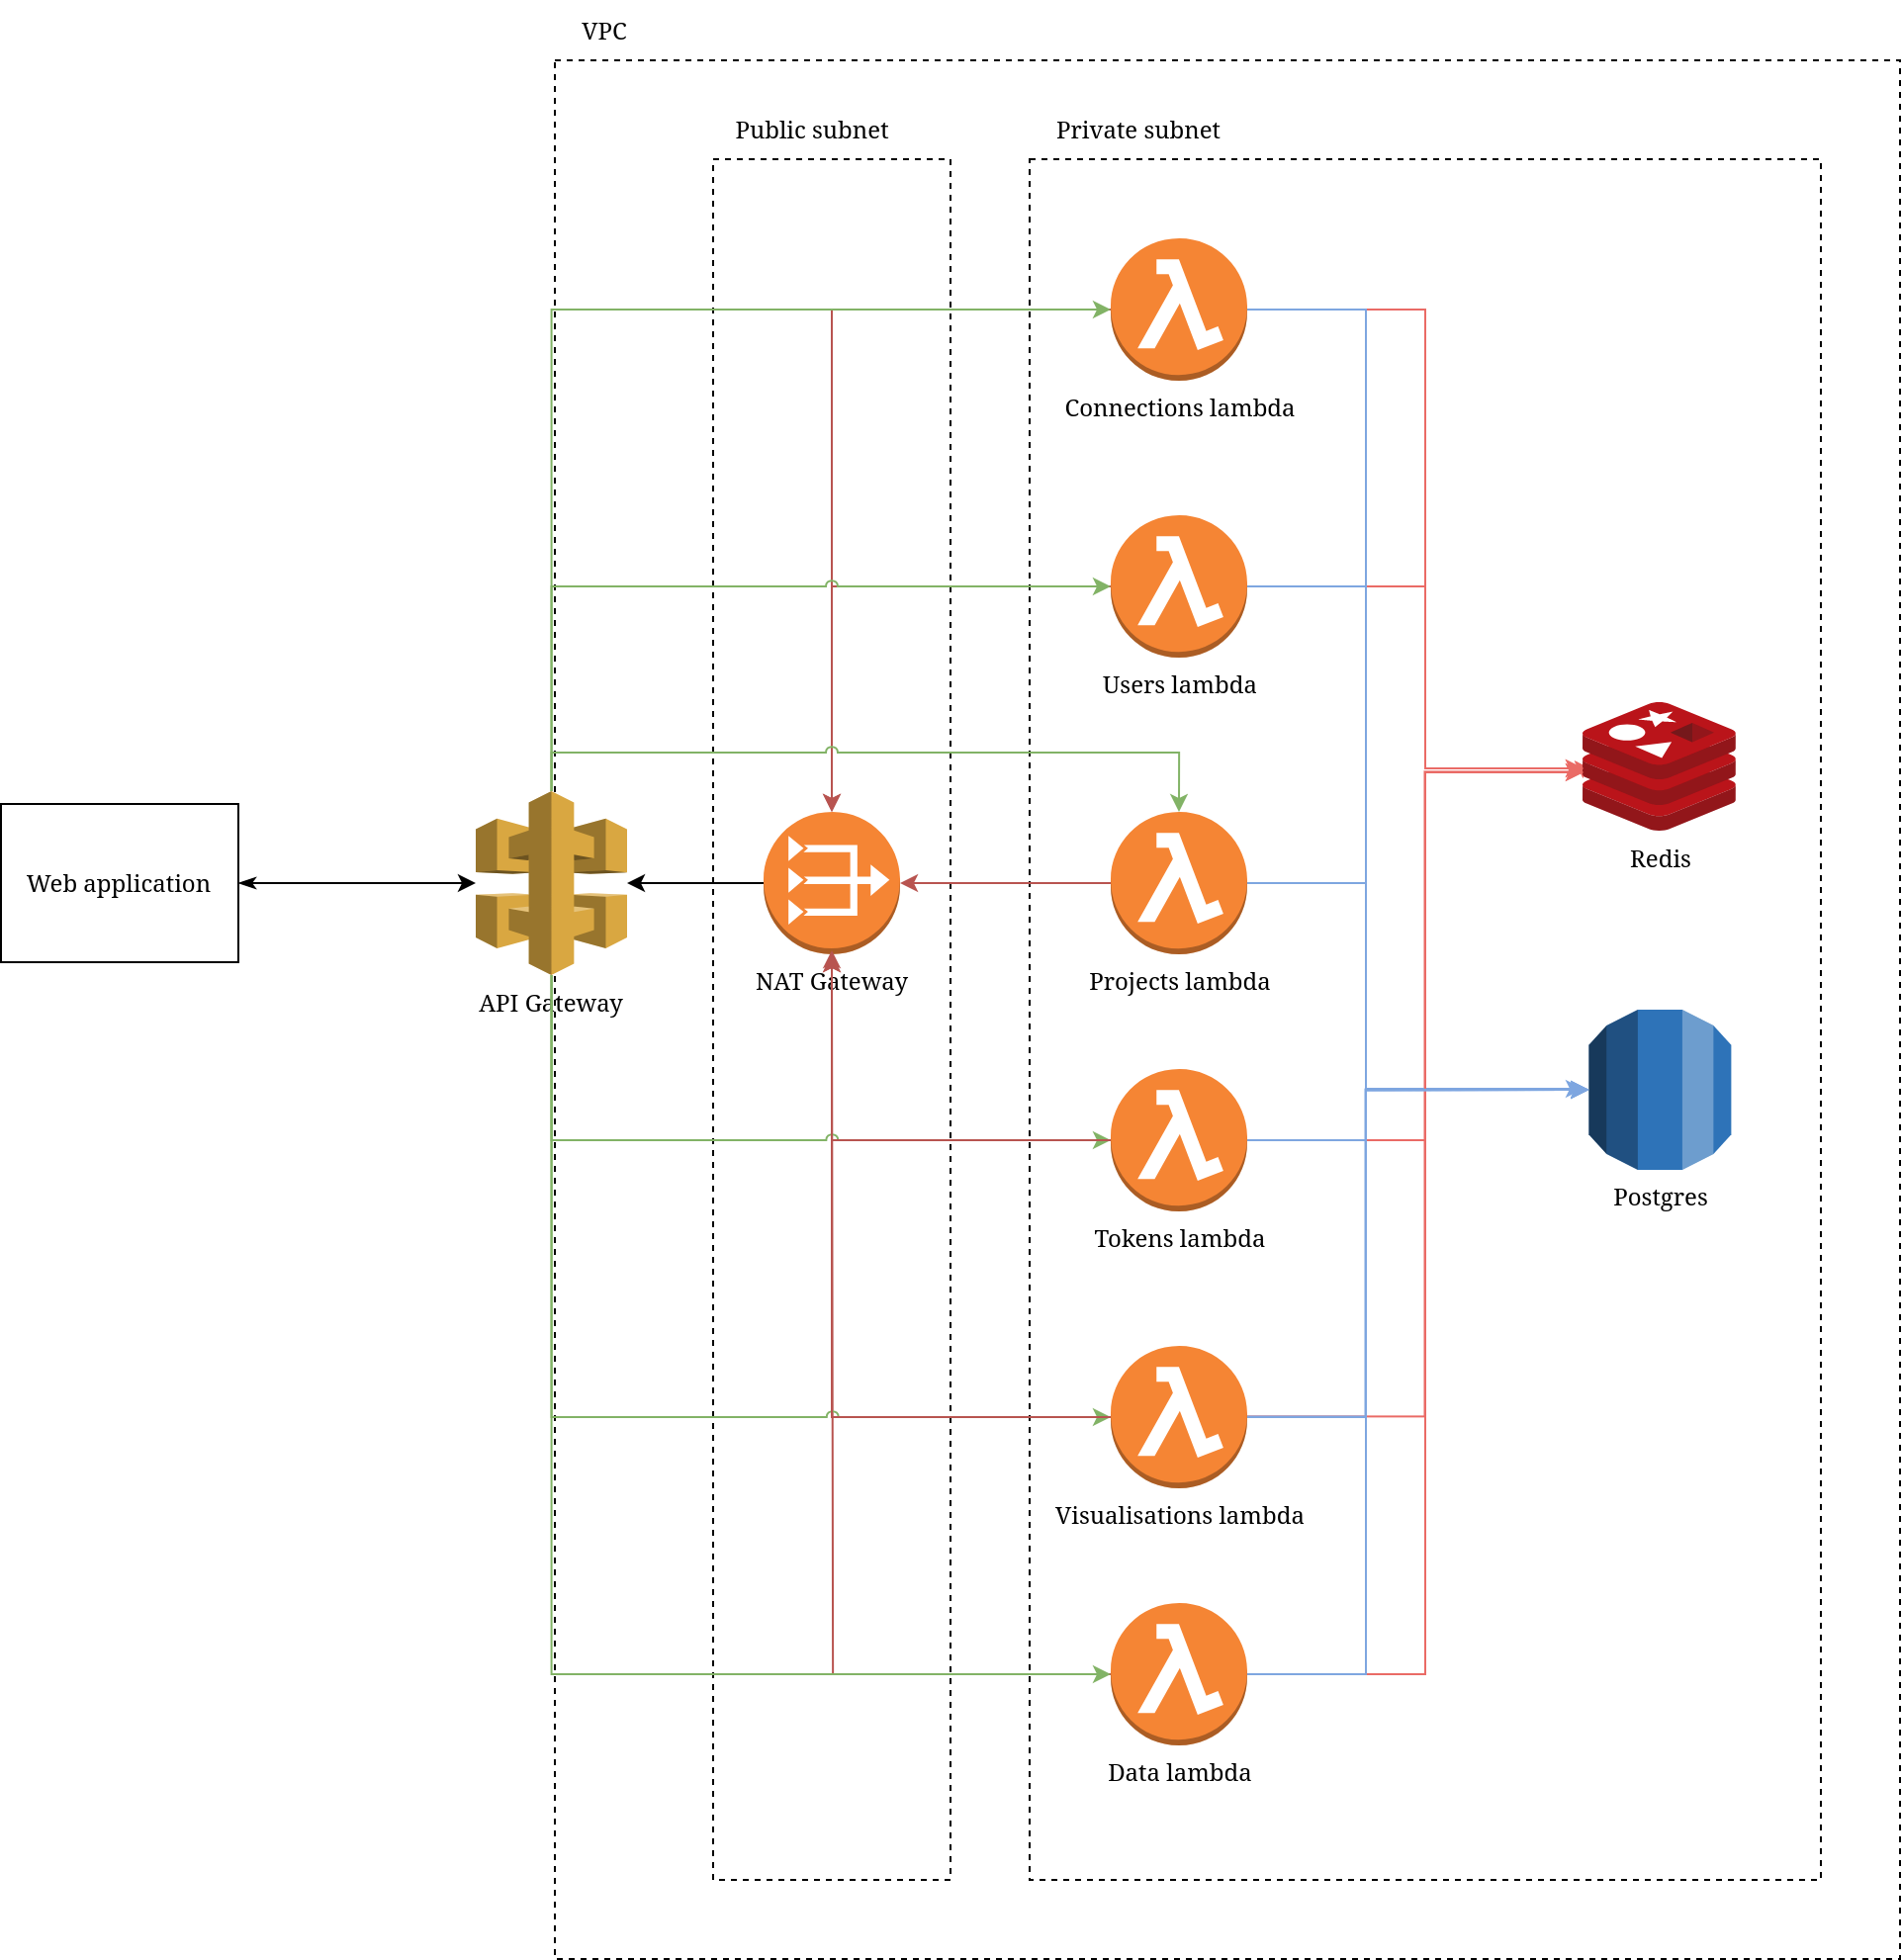
\includegraphics[width=0.7\textwidth]{pcd2.drawio.png}
    \caption{Architecture Diagram}
    \label{fig:diagrama}
\end{figure}

\section{Architecture}

\hspace{1cm} We designed a distributed system with a client-server architecture that provides scalability, modularity,
and effective resource management. The three main elements are:

\subsection{Client component}

\hspace{1cm}The user interface, which is in charge of facilitating direct communication with end users, is represented by the client component. The React web application acts as a representation of this in our scenario. The client program controls all aspects of record processing and result display, while the server processes requests from the client and returns results.

\subsection{Library component}

\hspace{1cm}We provide library clients currently for Node.JS and for web browsers.

\subsection{Server component}

\hspace{1cm}The backend of the application, which handles business logic, data processing, and storage, is represented by the server component. In this case, AWS services like Redis, Amazon RDS, API Gateway, and AWS Lambda represent this component. The client sends requests to the server, which uses business logic to process them and then sends the results back to the client.


\begin{itemize}
    \item \textbf{API Gateway with WebSockets}: Our API endpoints are managed by Amazon API Gateway, which also offers support for WebSocket communication. API Gateway WebSocket APIs are bidirectional.Services can send messages to clients on their own, and clients can send messages to services. Because of this bidirectional behavior, that allows services to push data to clients without explicitly requesting it, clients and the backend infrastructure can have richer interactions. 
    \item \textbf{AWS Lambda Functions}: According to the AWS documentation Lambda runs the code on a high-availability compute infrastructure and performs all of the administration of the compute resources, including server and operating system maintenance, capacity provisioning and automatic scaling, and logging. We use six AWS Lambda functions to handle various aspects of our application logic. These serverless functions provide scalable and economical processing by executing code in response to being triggered by events.
    \item \textbf{Redis}: Redis is an open-source network-connected in-memory cache that serves to speed up our application by caching frequently accessed information. It helps to lower latency for some processes by providing quick read and write operations.
    \item \textbf{Amazon RDS with PostgreSQL}: We use the relational database management system PostgreSQL with Amazon RDS for durable data storage. Our data is protected by this managed database service, which provides scalability, dependability, and automated backups for disaster recovery.
    \item \textbf{Virtual Private Cloud (VPC)}: In order to isolate our resources and offer better security, every component of our application is deployed inside a Virtual Private Cloud (VPC). This lets us specify the public and private subnets, routing tables, and IP ranges that compose our network environment.
\end{itemize}

\section{Analysis of System Characteristics}


\subsection{Performance}

\hspace{1cm} Our system uses independently-scalable Lambda functions for its entire compute stack.
The work necessary to process a resource is split between 6 lambda functions: connections, users, projects, tokens, visualisations and data.
The compute system is designed to be as horizontally scalable as possible.

\subsection{Latency}

\hspace{1cm} While testing, we measured the following request-response latencies:

\begin{table}[htbp]
    \centering
    \begin{tabular}{c|c c c}
        Unit & Min & Median & Max \\
        \hline
        Connections & 70ms & 92ms & 2374ms \\
        Users & 75ms & 85ms & 2526ms \\
        Projects & 72ms & 89ms & 2497ms \\
        Tokens & 114ms & 241ms & 2351ms \\
        Visualisations & 99ms & 130ms & 1952ms \\
        Data & 312ms & 642ms & 2129ms
    \end{tabular} 
    \caption{Latencies table}
\end{table}

The max times in the table above are mostly due to cold-start issues on the Lambda runtime side, which \textit{can be}
improved when using cold-startup mitigation strategies (polling the lambda function to keep warm, for instance).

\subsection{Costs}

\hspace{1cm}Since we run our stack using AWS Lambda, our application's costs are rather on the low side. The majority of
the costs are on the VPC NAT Gateway (included in EC2 below), RDS and Redis side.

\begin{table}[htbp]
    \centering
    \begin{tabular}{c|c}
        Unit & Cost \\
        \hline
        EC2 & 28.09 \\
        RDS & 12.70 \\
        ElastiCache & 9.77 \\
        VPC & 4.97 \\
        API Gateway & 0.17 \\
        S3 & 0.02
    \end{tabular} 
    \caption{Costs for ~3 weeks of usage}
\end{table}

\subsection{Reliability}

\hspace{1cm}Because of their automatic failover methods, frequent backups, and built-in redundancy, AWS services are highly reliable. While AWS Lambda offers fault tolerance with automatic scaling and replication across several availability zones, Amazon RDS guarantees data durability with automated backups and multi-AZ options for deployment.

\subsection{Monitoring transparency for developers}

\hspace{1cm}When building the application we extensively used CloudWatch to monitor the performance of our systems, detect
bottlenecks and pinpoint issues. Using these, WebSockete can promptly detect and resolve
problems thanks to these transparency features, which guarantees the dependability and availability of our
program.

\section{Points of improvement}

\hspace{1cm}During the development of the application, we noted down some points of improvement, some of them being:

\begin{enumerate}
    \item Switch from Lambda to ECS in order to improve latency further, as the application requires more realtime data processing
    \item Add sharding for RDS to improve performance
    \item Implement Redis clustering
    \item Distribute our web application using CloudFront CDN
    \item Improve presentation layer by adding graphs, i18n, user settings, data sharing
    \item Add more features to the presentation layer (maybe logs?)
\end{enumerate}

\section{Conclusions}

\hspace{1cm}In conclusion, despite the fact that our application is still in its early stages of development, we have built a strong basis for creating a reliable and effective distributed application. Our architectural approach makes use of AWS's scalability, stability, and security characteristics. Future development paths can include optimizing security by encrypting sensitive data using AWS Key Management Service (KMS) and performance by using AWS Auto Scaling to automatically modify computing power to manage variable amounts of demand.

\end{document}
